\chapter[Apéndice]{
  \label{chp:apendice}
  Demostración
}

En este apéndice se mostrará el funcionamiento de la aplicación, primero con
la versión para computador y a continuación la aplicación web. Para ello, se
mostrará el caso de uso para generar una presentación KML. No se
pretende detallar todos los parámetros del proceso, puesto que están cubiertos 
por la documentación de usuario disponible en la web, sólo mostrar la 
apariencia de la aplicación y su filosofía de funcionamiento.

\section{\software}

Como se ha comentado, el proyecto ha sido desarrollado en abierto usando
la plataforma Google Code. El nombre elegido para el software ha sido
\software\footnote{Web oficial del proyecto \url{https://code.google.com/p/photoplace}} 
y se ha desarrollado un logotipo que refuerza la identidad del programa:

\begin{figure}[H]
  \centering
  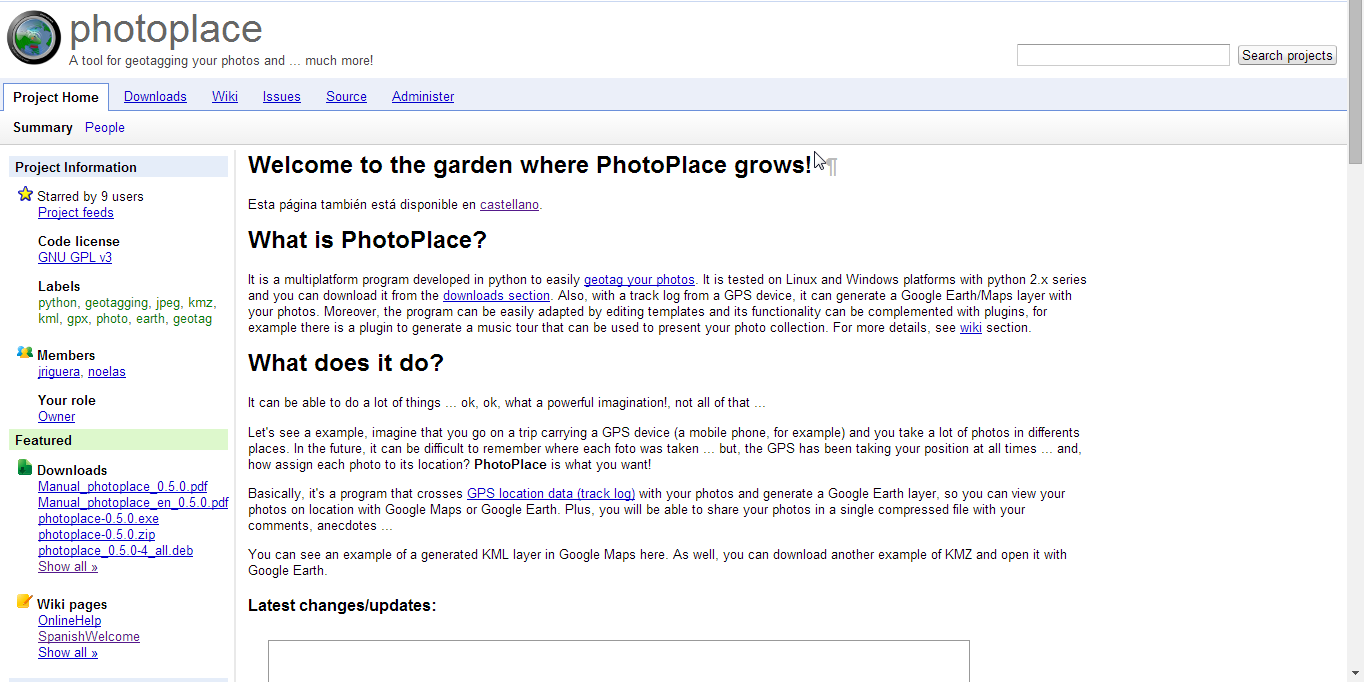
\includegraphics[scale=0.4,keepaspectratio=true]{photoplace.png}
  \caption*{Web de desarrollo de \software\ en Google Code}
  \label{fig:photoplace}
\end{figure}
